\documentclass[14pt]{article}
\usepackage[utf8]{vietnam}
\usepackage{graphicx}
\usepackage{listings}
\graphicspath{ {figures/} }
\usepackage{fancyhdr}
\usepackage{geometry}
\usepackage{float}
\usepackage[bottom]{footmisc}
\usepackage{afterpage}
\usepackage{multirow}
\usepackage[table]{xcolor}
\definecolor{highlight}{RGB}{230, 230, 230}
%\newcommand{\kb}{\textit{KB/s}}
%\newcommand{\kbs}{\textit{Kbps}}
%\newcommand{\mbs}{\textit{Mbps}}
%\newcommand{\gbs}{\textit{Gbps}}
%\newcommand{\mb}{\textit{MB/s}}

\lstset{numbers=left, numberstyle=\tiny, stepnumber=2, numbersep=5pt, tabsize=2, language=java, basicstyle=\small}
\newcommand\blankpage{%
    \null
    \thispagestyle{empty}%
    \addtocounter{page}{-1}%
    \newpage}
\geometry{
	left=2cm, right=2cm,
	top=2cm, bottom=2cm,
	includefoot=true,
	includehead=true,
	headsep = 40pt,
}
% create the header for this file
\pagestyle{fancy}
\begin{document}
\thispagestyle{empty}


\fancyhead{} % clear all header fields
\fancyhead[L]{
 \begin{tabular}{rl}
    \begin{picture}(25,15)(0,0)
    \put(0,-8){
\includegraphics[width=8mm, height=8mm]{Images/hcmut.pdf}}
   \end{picture}&
	\begin{tabular}{l}
		\textbf{\bf Đại học Bách Khoa Tp. Hồ Chí Mính}\\
		\textbf{\bf Khoa Khoa học \& Kỹ thuật Máy Tính}
	\end{tabular} 	
 \end{tabular}
}

\fancyfoot{} % clear all footer fields
\fancyfoot[L]{\scriptsize Báo cáo bài tập lớn số 2}
\fancyfoot[R]{\scriptsize \thepage}
\renewcommand{\headrulewidth}{0.3pt}
\renewcommand{\footrulewidth}{0.3pt}

\begin{center}
\LARGE\bfseries ĐẠI HỌC QUỐC GIA TP HỒ CHÍ MINH \\
TRƯỜNG ĐẠI HỌC BÁCH KHOA \\

\end{center}
\begin{center}
\LARGE\bfseries 
Khoa Khoa Học \& Kỹ Thuật Máy Tính
\end{center}
\begin{center}

\includegraphics[scale=0.2]{Images/hcmut.pdf}\\[1cm]
\end{center}

\vspace{1cm}

\begin{flushleft}
\Large \bfseries TRÍ TUỆ NHÂN TẠO\\
Bài tập lớn số 2\\[0.5cm]
\end{flushleft}
\rule{\textwidth}{1pt}
\vspace{2pt}
\begin{center}
\huge
\begin{tabular}{@{}l}
ROBOCODE\\[10pt]
\end{tabular}
\end{center}
\rule{\textwidth}{1pt}\\[1cm]

\vspace{1cm}

\begin{minipage}[t]{0.60\linewidth}
\textbf{GVHD}: \\
Gs. Cao Hoàng Trụ\\
Ths. Vương Bá Thịnh

\end{minipage}
\begin{minipage}[t]{0.25\linewidth}
\textbf{NHÓM Feederz:}\\
Nguyễn Kim Trung Hiếu\\
Đỗ Nguyễn Khánh Hoàng\\
\end{minipage}
\begin{minipage}[t]{0.20\linewidth}
\textbf{}\\
51201097\\
51201200\\
\end{minipage}
\begin{center}

\vspace{2cm}
{Tp. HCM, 05/2015}

\end{center}

\newpage
\thispagestyle{empty}
\emph{ }
\newpage
\thispagestyle{empty}
\tableofcontents
\thispagestyle{empty}

\newpage
\thispagestyle{empty}
\listoffigures

\newpage
\thispagestyle{empty}
\begin{center}
This page intentionally left blank
\end{center}
\newpage
\section{Robocodde}
\subsection{Giới thiệu}
\subsection{Luật chơi}
\section{Tổ chức Class}
Chương trình được tổ chức rõ ràng với 04 class chính. Nhiệm vụ mỗi class được phân chia cụ thể và hợp lý.
\begin{figure}[H]
\centering
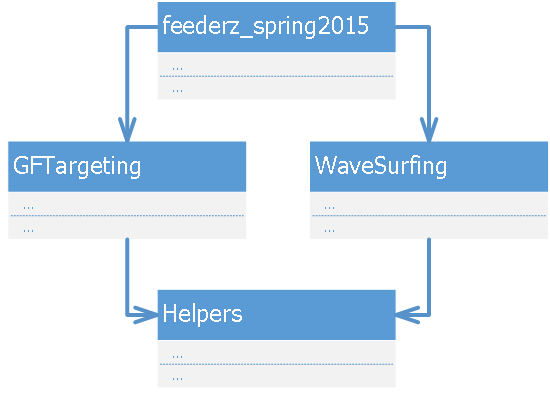
\includegraphics[scale=0.5]{images/classStructrure.png}
\caption{Tổ chức class}
\end{figure}
\begin{itemize}
	\item \textbf{feederz\_spring2015}: class chính hiện thực robot. Ở đây chứa các hàm cơ bản mà hệ thống sẽ gọi trong suốt quá trình robot chạy
	\item \textbf{WaveSurfing}: class hiện thực kỹ thuật Wave Surfing, chịu trách nhiệm tính toán và điều khiển đường đi của robot, né đạn và né tường
	\item \textbf{GFTargeting}: class hiện thực kỹ thuật Guess Factor, chịu trách nhiệm tính toán và điều khiển súng của robot để nhắm chính xác mục tiêu
	\item \textbf{Helpers} class chứa các hàm bổ trợ được sử dụng bởi các class trên
\end{itemize}
\section{Kỹ thuật Wall Smoothing}
Theo luật của robocode, mỗi lần va chạm với tường robot cũng bị mất năng lượng giống như khi bị trúng đạn. Hơn nữa, nếu robot va chạm với tường và mắc kẹt ở một trong bốn góc của sân đấu thì khả năng bị tiêu diệt sớm lại càng cao hơn. Do vậy, để nâng cao khả năng sống còn của robot, việc đầu tiên cần nghĩ ngay tới đó là làm cho robot "né" được tường trong lúc chiến đấu, đừng để nó di chuyển vào những điểm chết hoặc những điểm quá gần tường.

Đầu tiên ta thiết lập một vùng an toàn cho robot. Trong suốt trận đấu, ta cố gắng điều khiển cho robot di chuyển không vượt qua giới hạn của vùng này. Cụ thể, kích thước vùng này được quy định bởi một hình chữ nhật \textit{playingRectangle} như trong source code.
\begin{lstlisting}[caption = Thiết lập vùng an toàn, frame = single]
public static final int BATTLEFIELD_WIDTH = 8100;
public static final int BATTLEFIELD_HEIGHT = 600;
static final int BOUNDARY_SIZE = 18;
public static Rectangle2D.Double playingRectangle = new Rectangle2D.Double(
		BOUNDARY_SIZE, BOUNDARY_SIZE,
		BATTLEFIELD_WIDTH - BOUNDARY_SIZE * 2, 
		BATTLEFIELD_HEIGHT - BOUNDARY_SIZE * 2);
\end{lstlisting}
Kích thước cố định của sân đấu là $800 \times 600$. Vùng an toàn là hình chữ nhật nhỏ bên trong, cách biên của sân đấu một khoảng BOUNDARY\_SIZE = 18.

Xử lý va chạm với tường được giải quyết bằng kỹ thuật Wall Smoothing. Giải thuật này cố gắng tìm ra một góc gọi là "an toàn", nghĩa là nếu robode tiến theo góc đó thì nó không thể va chạm với tường đồng thời cũng không di chuyển quá gần về phía đối thủ.
\begin{lstlisting}[caption = wallSmoothing function, frame = single]
public double wallSmoothing(Point2D.Double botLocation, double angle,int orientation) {
	Point2D.Double guesingPosition = 
									Helpers.getPositionFromAngleAndDistance(botLocation, angle, WALL_STICK);
	while (!playingRectangle.contains(guesingPosition)) {
		angle += orientation * 0.05;
		guesingPosition = Helpers.
			getPositionFromAngleAndDistance(botLocation, angle, WALL_STICK);
	}
	return angle;
}
\end{lstlisting}
Hàm wallSmoothing cần biết 03 thông tin để có thể xác định được góc đi an toàn tiếp là góc nào. Chúng là:
	\begin{itemize}
		\item Vị trí hiện tại của robot
		\item Góc đi vuông góc. Thật khó trình bày bằng lời góc này xác định như thế nào. Tuy nhiên nhiên nếu nhìn vào hình vẽ ta thấy, để đi vuông góc với phương nối giữa robot và enemy, robot phải đi theo hướng $P_1$. Và góc \textit{angle} chính là góc tương đối giữa mũi tên $P_1$ với trục đứng chỉ $0^o$, tức góc $\alpha$. Vì góc này nằm bên trái trục $0^o$ nên nó sẽ có giá trị âm.
		\item Hướng di chuyển hiện tại. Nếu chọn enemy làm tâm thì robot có 02 hướng chính để di chuyển là theo chiều kim đồng hồ và ngược chiều kim đồng hồ tướng ứng với giá trị +1 và -1 của \textit{orientation}. Như trong hình vẽ, robot đang di chuyển theo hướng thuận chiều kim đồng hồ nên giá trị này sẽ là +1.
	\end{itemize}
Để hiểu rõ cách hoạt động của giải thuật này, ta sẽ xét trường hợp trong hình. Theo đó nếu đi theo góc $\alpha$ thì sau một đoạn đường WALL\_STICK = 160, vị trí của robot là $P_1$ - tức nằm trong vùng nguy hiểm. Giải thuật sẽ cố gắng xoay mũi tên này vào sâu trong sân đấu để vị trí mới này nằm trong vùng an toàn, đồng thời góc này phải hướng ra xa enemy lớn nhất có thể. Và do đó, mũi tên này sẽ quay vào trong và dừng lại khi đạt góc $\beta$ tương ứng với vị trí $P_2$. Cứ như vậy, giải thuật sẽ luôn hướng góc di chuyển của robot vào trong sân đấu và giữ khoảng cách an toàn đối với tường.
\begin{figure}[H]
\centering
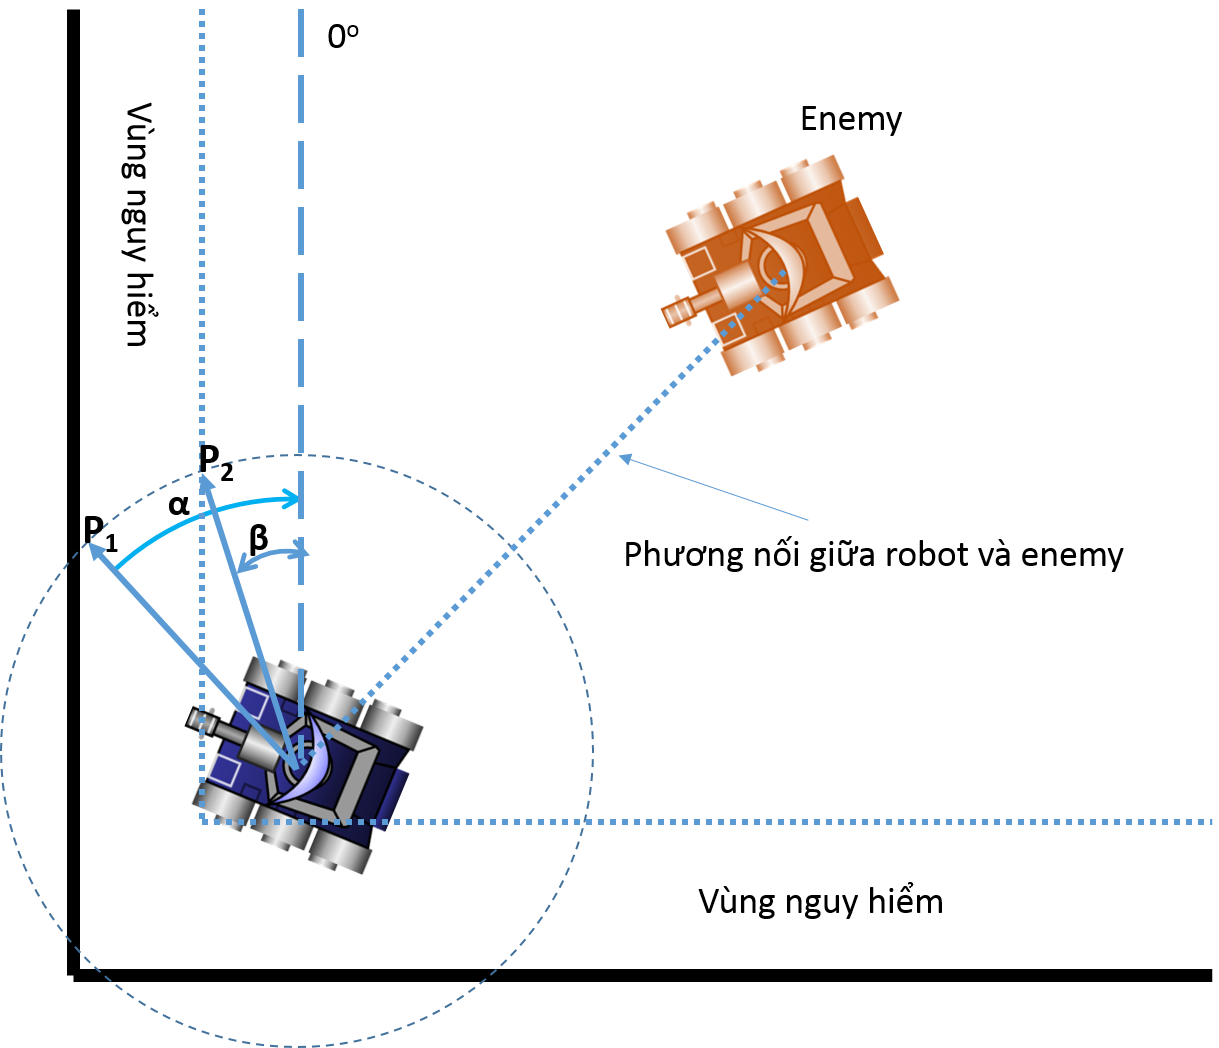
\includegraphics[scale=0.5]{images/wallsmoothing.png}
\caption{Kỹ thuật Wall Smoothing}
\end{figure}
\section{Kỹ thuật Wave Surfing}
\subsection{Giới thiệu}
Một đội chơi đến từ Bồ Đào Nha tên là ABC là những người đầu tiên mang kỹ thuật Wave Surfing vào sử dụng khi họ áp dụng để phát triển robot Shadow vào giữa năm 2004. Cho đến tháng 4 năm 2010, top 40 đội đứng đầu đều sử dụng những dạng biến thể của nó để phát triển robot cho mình. Mấu chốt của kỹ thuật này đó là việc xác định thời điểm đối phương bắn đạn để từ đó dự đoán mục tiêu của nó. Càng nhiều thông tin thu thập được sau mỗi phát bắn, khả năng dự đoán vùng nguy hiểm, tức vùng mà đối phương thường nhắm vào, càng chính xác hơn, để từ đó lựa chọn những đường đi phù hợp.
\subsection{Trừu tượng hóa thông tin đạn bắn}
Để tiện cho việc quản lý, những thông tin về đạn được thu thập, tổ chức và quản lý theo từng wave. EnemyWave là một đối tượng trừu tượng dùng để đóng gói thông tin một viên đạn bắn ra. Chúng bao gồm:
	\begin{itemize}
		\item fireLocation: vị trí mà ở đó viên đạn được bắn ra.
		\item fireTime: thời điểm bắn đạn
		\item bulletVelocity: vận tốc của viên đạn
		\item directAngle: góc bắn
		\item distanceTraveled: khoảng cách viên đạn đã đi được, tính từ fireLocation
		\item direction: hướng bắn
	\end{itemize}
\begin{lstlisting}[caption = EnemyWave, frame = single]
class EnemyWave {
	Point2D.Double fireLocation;
	long fireTime;
	double bulletVelocity, directAngle, distanceTraveled;
	int direction;

	public EnemyWave() {}
}
\end{lstlisting}
\begin{figure}[H]
\centering
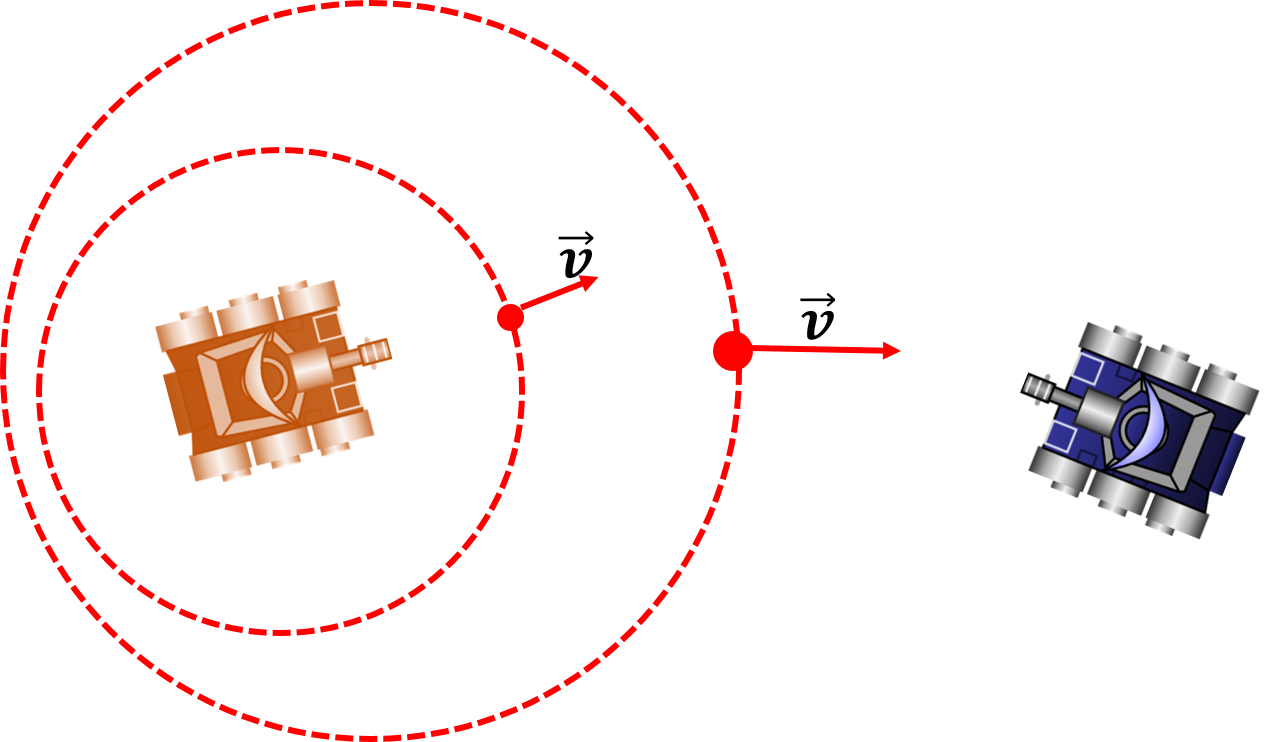
\includegraphics[scale=0.5]{images/wavesurfing_introduction.png}
\caption{EnemyWave}
\end{figure}
\subsection{Nhận biết thời điểm bắn đạn}
API của robocode không cung cấp sự kiện nào để nhận biết việc bắn đạn. Tuy nhiên chúng ta có thể xác đinh được điều này thông qua sự sụt giảm năng lượng của đối phương. Như đã biết, mỗi lần bắn đạn robot sẽ bị mất một khoảng năng lượng và lượng thâm hụt $deltaEnergy$ này thỏa mãn $0 < deltaEnergy \leq 3.0$. Mỗi khi radar phát hiện được đối phương có dấu hiệu này thì chương trình khởi tạo một EnemyWave mới. Việc dự đoán này không phải lúc nào cũng chính xác 100\% và các cải thiện sẽ được trình bày trong những phần sau.
\subsection{Phân chia phạm vi nguy hiểm}
Mỗi khi robot bị trúng đạn, thông tin của viên đạn được truy xuất để phục vụ cho việc phân hoạch vùng nguy hiểm. Việc phân hoạch này có thể dựa trên nhiều yếu tố bao gồm cả vận tốc đạn, khoảng cách đạn hoặc là góc bắn. Tuy nhiên vì chương trình khá đơn giản nên chúng em chỉ hiện thực phân hoạch dựa trên góc bắn. 
\begin{figure}[H]
\centering
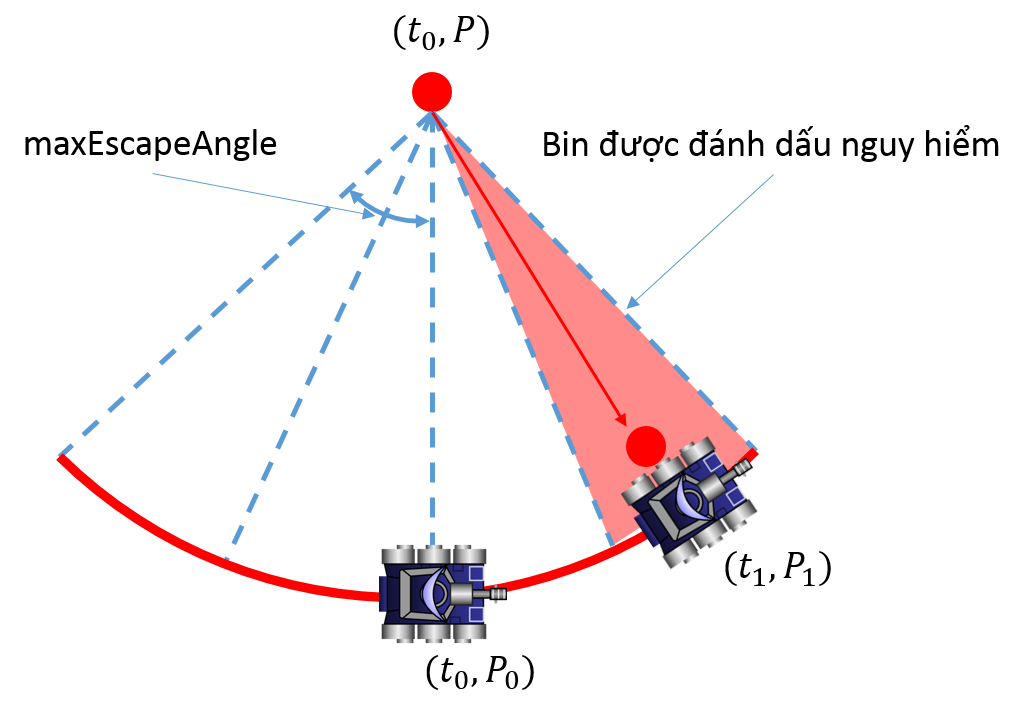
\includegraphics[scale=0.5]{images/segmentation.png}
\caption{Phân hoạch vùng nguy hiểm}
\end{figure}
Theo đó ứng với mỗi EnemyWave, hoặc nói theo cách khác là ứng với mỗi viên đạn được bắn ra, chúng ta sẽ xác định được một góc bắn như hình vẽ. Góc này có độ lớn bằng 2 lần góc maxEscapeAnlge\footnote{Là góc lớn nhất mà robot có thể di chuyển được trong một đơn vị thời gian - một tick. Việc giới hạn này là hợp lý vì mọi góc nằm ngoài khoảng này là không cần xem xét vì robot không thể nào di chuyển tới đó được} và được chia ra thành những phần bằng nhau được gọi là BIN. Trong chương trình sử dụng 47 BIN còn trong hình minh họa thì chia ra được 4 BIN. Một BIN được đánh dấu là nguy hiểm nếu như robot bị trúng đạn khi đang di chuyển trong BIN đó. Chẳng hạn như trong hình vẽ, tại thời điểm $t_0$ robot đang ở vị trí $P_0$ và nhận thấy đối thủ bắn ra viên đạn tại ví trí $P$. Cho đến thời điểm $t_1$ robot bị viên đạn đó đụng phải tại vị trí $P_1$ - thuộc BIN thứ 4. BIN này được tô đỏ trong hình vẽ và nghĩa là trong tương lai, nếu gặp trường hợp tương tự như vậy, robot sẽ hạn chế di chuyển vào BIN này. Tất cả các bị này được tổ chức và lưu trong biến statArray[].

Theo cách đánh dấu như vậy, càng về sau, sự phân hoạch vùng nguy hiểm này sẽ càng chính xác, và robot sẽ học được chiến lược bắn đạn của đối phương để tìm đường đi an toàn cho mình.
\subsection{Kiểm tra mức nguy hiểm}
Mỗi khi nhận biết một viên đạn đang bay tới gần, chương trình sẽ tiến hành kiểm tra xem mức độ nguy hiểm của hướng mình đang đi, nghĩa là xác định xem, nếu cứ tiếp tục đi như vậy thì khả năng viện đạn này va chạm robot cao đến mức nào. Sự đánh giá này dựa trên những thông tin thu thập được từ các BIN trong statArray. Hàm checkDanger sẽ làm công việc đó.
\begin{lstlisting}[caption = checkDanger, frame = single]
public double checkDanger(EnemyWave surfWave, int direction) {
	int index = calculateIndex(surfWave,
			predictPosition(surfWave, direction));
	return statArray[index];
}
\end{lstlisting}
Từ thông tin về viên đạn sắp tới surfWave và hướng đi chuyển hiện tại direction hàm dự đoán vị trí của robot bằng predictPosition và tính toán hệ số của BIN cần tìm. Sau đó trả về giá trị của BIN này trong statArray.
\subsection{Chọn hướng đi an toàn}
Việc lựa chọn này chỉ dựa trên thông tin của viên đạn gần nhất comingWave. Hàm tiến hành kiểm tra mức nguy hiểm của hai hướng đi trái phải (ngược chiều, cùng chiều kim đồng hồ). Sau khi lựa chọn được một hướng đi an toàn nhất, góc tìm được sẽ được xử lý bởi hàm wallSmoothing để tránh trường hợp đụng tường. Góc goAngle trả về là góc cuối cùng mà robot sẽ luôn định hướng đi theo trong suốt chương trình.
\begin{lstlisting}[caption = getPerfectAngleToGo, frame = single]
public double getPerfectAngleToGo() {
	EnemyWave comingWave = getClosestSurfableWave();
	if (comingWave == null) {
		return Double.POSITIVE_INFINITY;
	}
	double dangerLeft = checkDanger(comingWave, -1);
	double dangerRight = checkDanger(comingWave, 1);

	double goAngle = Helpers.getAbsoluteBearingAngle(
			comingWave.fireLocation, ourRobotPosition);
	if (dangerLeft < dangerRight) {
		goAngle = wallSmoothing(ourRobotPosition, goAngle - (Math.PI / 2),
				-1);
	} else {
		goAngle = wallSmoothing(ourRobotPosition, goAngle + (Math.PI / 2),
				1);
	}
	return goAngle;
}
\end{lstlisting}
\subsection{Những biện pháp cải tiến}
{\bf Giữ khoảng cách cố định}\\
Chương trình không quan tâm đến việc giữ khoảng cách tương đối giữa robot và enemy. Nếu cải thiện được thì việc dự đoán đạn của robot sẽ chính xác hơn.\\
{\bf Theo dõi năng lượng của đối thủ chính xác hơn}\\
Như đã trình bày ở phần trước, mỗi lần phát hiện ra đối thủ mất một mức năng lượng $0 < p \leq 3.0$ thì robot sẽ ghi nhận một viện đạn được bắn ra. Cách dự đoán này tuy đa phần chính xác những có một số trường hợp ngoại lệ, đặc biệt là khi gần kết thúc trận đấu - cả hai đều bắn đi những viên đạn có năng lượng nhỏ. Nói là không chính xác bởi vì không phải lúc nào đối thủ mất năng lượng cũng đều do bắn đạn. Đó có thể là do nó bị trúng đạn của ta bắn. Trong trường hợp đó, data thu thập được sẽ bị sai do những "viên đạn ảo" này, ảnh hưởng đến khả năng dự đoán.\\
{\bf Thay đổi chiến lược né đạn}\\
Hiện tại ý tưởng né đạn vẫn là xác định xem viên đạn nào di chuyển đến gần robot nhất để né. Giải pháp này không hiệu quả bằng việc xem xét né viên đạn sẽ chạm robot trước thay vì viên gần nhất.
\section{Guess Factor}
\section{Javadoc}
\subsection{Class WaveSurfing}
\begin{tabular}{|p{4cm}|p{6cm}|p{6cm}|}
\hline
\bf Tên hàm&\bf Parameters&\bf Giải thích\\
\hline
WaveSurfing&robot: Đối tượng robot cần điều kiển di chuyển& Hàm constructor của class WaveSurfing\\
\hline
getPerfectAngleToGo&@return: góc (radian)& Xác định góc an toàn nhất để đi, có xét đến việc tránh đạn cũng như tránh tường\\
\hline
updateData&e: đối tượng thuộc sự kiện ScannedRobotEvent&Dựa vào những thông tin có được từ đối tượng ScannedRobotEvent, tiến hành cập nhật:
	\begin{itemize}
		\item Vị trí hiện tại của robot
		\item Hướng di chuyển
		\item Góc nhắm của enemy vào robot
		\item Tạo EnemyWave mới nếu phát hiện đạn được bắn ra
	\end{itemize}\\
\hline
onBulletHit&e: đối tượng BulletHitEvent& Cập nhật thông tin về thời điểm đạn của mình bắn trúng đối phương, phục vụ cho quá trình dự đoán xuất hiện EnemyWave\\
\hline
onHitByBullet&e: đối tượng HitByBulletEvent& Cập nhật thông tin về viên đạn của đối phương bắn trúng mình. Những dữ liệu này được sử dụng để tính toán lại mức độ nguy hiểm (cập nhật lại giá trị trong các BIN)\\
\hline

\end{tabular}

\subsubsection*{Thông tin các thuộc tính}

\begin{tabular}{llp{9cm}}
\textbf{ourRobot}&AdvancedRobot&Đối tượng robot được truyền vào để điều khiển\\
\textbf{ourRobotPosition}&Point2D&Vị trí hiện tại của robot\\
\textbf{enemyPosition}&Point2D&Vị trí hiện tại của đối thủ\\
enemyWaves&ArrayList<EnemyWave>&List các đối tượng EnemyWave chứa thông tin về các viên đạn của đối thủ bắn ra\\
directionArray&ArrayList<Integer>&List chứa các hướng di chuyển của robot theo thời gian\\
BINS&int&Số lượng BIN tối đa được chia ra\\
statArray&double[]&Dãy chứa các giá trị của các BIN\\
absBearingsArray&ArrayList<Double>&Chứa các góc ngắm tuyệt đối của đối thủ (radian)\\
\end{tabular}

\subsubsection{Thông tin các hàm}
\textbf{WaveSurfing}\\
	\begin{description}
		\item public WaveSurfing(AdvancedRobot robot)
		\item Khởi tạo đối tượng WaveSurfing
		\item Parameters:
		\begin{description}
				\item[robot] - đối tượng robot cần gán điều khiển di chuyển
			\end{description}
	\end{description}
\vspace{0.5cm}
\textbf{getPerfectAngleToGo}
	\begin{description}
		\item public double getPerfectAngleToGo()
		\item Chọn góc đi phù hợp nhất, có xét đến cả sự đụng tường và né đạn
		\item Returns: Góc đi (radian)
	\end{description}

\end{document}